\clearpage
\appendix
\section*{Appendix}
\addcontentsline{toc}{section}{Appendix}

\section{Numerical validation against the reference implementation}
\label{app:validation}

Every stage of the sensory pipeline is checked against the original NumPy code
in double precision on random scenes (\texttt{scripts/validate\_physics.py}).
Agreement is at floating-point round-off, and the knollenorgan and ampullary
pathways agree bit-for-bit.

% auto-generated by scripts/figures.py
\begin{table}[t]
\centering\small
\caption{Agreement between the GPU reimplementation and the reference NumPy implementation, in double precision on random scenes. Error is the maximum absolute deviation normalised by the largest magnitude present.}
\label{tab:validation}
\begin{tabular}{lr}
\toprule
Stage & Max. relative deviation \\
\midrule
Coulomb field of point charges & $\num{2.3e-15}$ \\
Field of point dipoles & $\num{1.4e-14}$ \\
Field including first-order wall images & $\num{1.9e-15}$ \\
Dipoles induced on conductors & $\num{1.2e-15}$ \\
Charge-limiting of fish body moments & $\num{1.2e-15}$ \\
Corollary-discharge baseline & $\num{1.6e-14}$ \\
Ampullary intrinsic baseline & $\num{1.3e-14}$ \\
Mormyromast, self-image mode & $\num{6.0e-10}$ \\
Mormyromast, collective-sensing mode & $\num{4.9e-11}$ \\
Knollenorgan (conspecific detection) & exact (0) \\
Ampullary (passive DC) & exact (0) \\
\bottomrule
\end{tabular}
\end{table}


\begin{figure}[h]
\centering
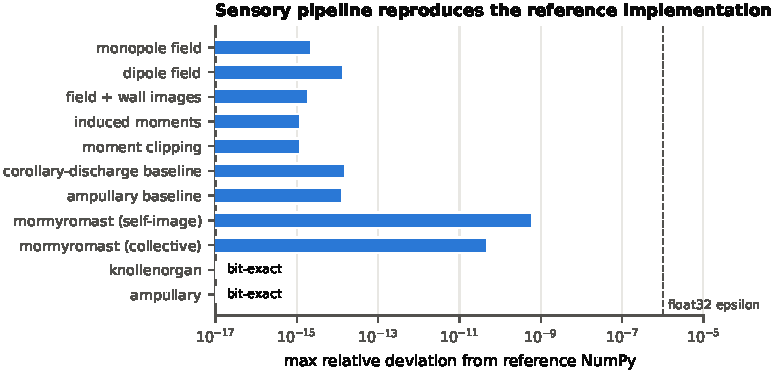
\includegraphics[width=0.62\textwidth]{../figs/fig1_validation.pdf}
\caption{Maximum relative deviation from the reference NumPy implementation over
random scenes, in double precision. Bars at the left edge are exactly zero.}
\label{fig:validation}
\end{figure}

\paragraph{An incidental bug in the reference code.} Its configuration file sets
a wall-reflection coefficient of $0.95$, but \texttt{ElectricScene.\_build\_%
reflections} never forwards it to \texttt{reflect\_sources}, whose default is
$1.0$. The published results therefore use unattenuated first-order images. We
match the code rather than the configuration file; using $0.95$ shifts the
corollary-discharge baseline by $\sim\num{1.4e-6}$ relative and changes ampullary
readings qualitatively, because those are a small difference of large numbers.

\section{Training the three channel conditions from scratch}
\label{app:scratch}

Training is bimodal: a seed either discovers patch foraging or stays near the
floor set by passive sensing alone. A seed counts as converged if it reaches half
the ceiling of its own task family, a criterion applied identically to every
condition within a family; the fraction clearing it is reported as its own
outcome, because conditions that remove sensory channels are not only worse on
average but less reliably learnable.

\begin{figure}[h]
\centering
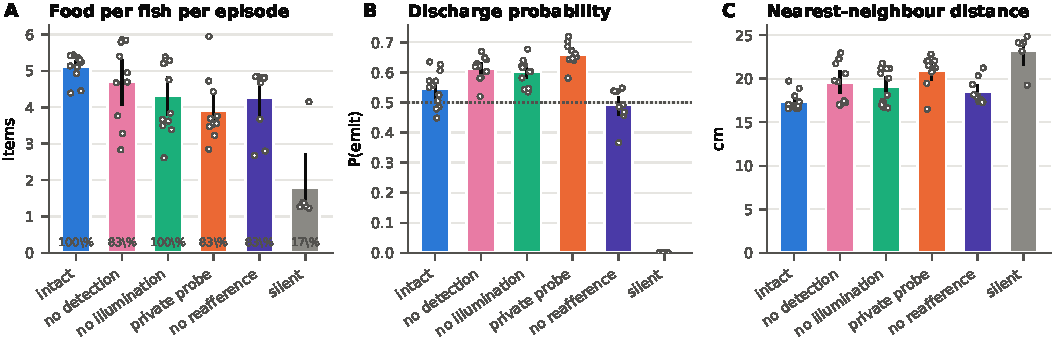
\includegraphics[width=\textwidth]{../figs/fig2_channels_scratch.pdf}
\caption{Removing each consequence of a discharge, trained from scratch. Bars are
means over independent seeds with bootstrap 95\% CIs; points are seeds.
Percentages in (A) give the fraction of seeds reaching the learning criterion.}
\label{fig:scratch}
\end{figure}

\section{Regime classification}
\label{app:regimes}

\begin{figure}[h]
\centering
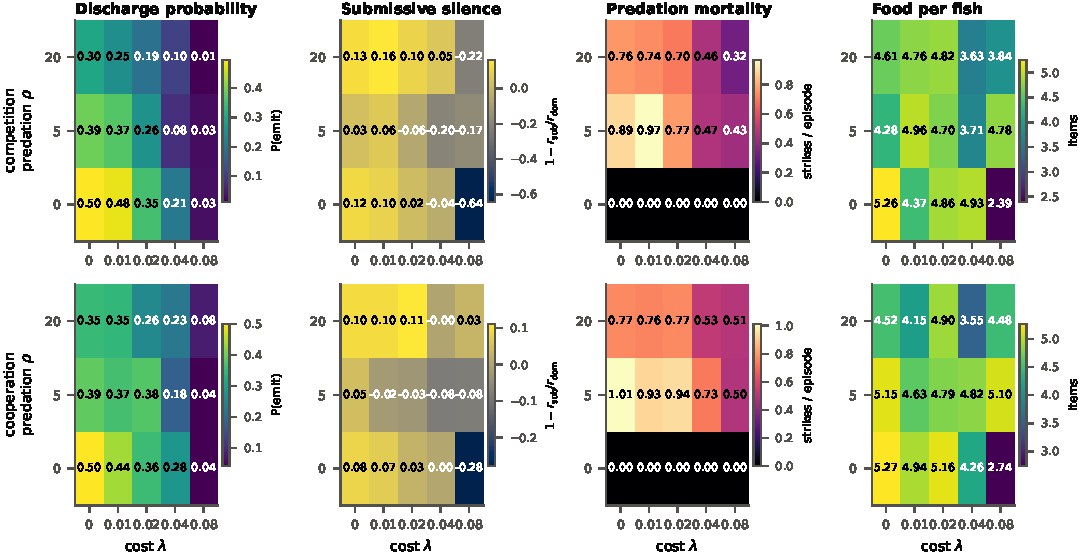
\includegraphics[width=\textwidth]{../figs/fig7_phase_grid.pdf}
\caption{Metabolic cost and eavesdropping predation jointly set discharge policy.
Rows are competitive and cooperative harvests; each cell is a mean over
independent seeds.}
\label{fig:phase}
\end{figure}

\begin{figure}[h]
\centering
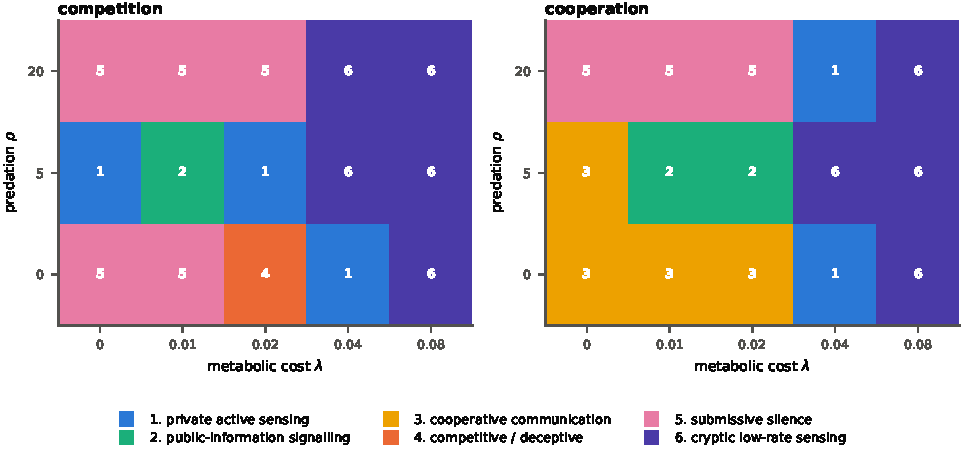
\includegraphics[width=0.92\textwidth]{../figs/fig8_regimes.pdf}
\caption{Rule-based regime labels from the pooled metric vector. Thresholds are
percentiles of each metric's own distribution across the grid rather than
hand-set values, so the boundaries describe a continuum and are not claims about
sharp transitions.}
\label{fig:regimes}
\end{figure}

\section{Limitations in full}
\label{app:limitations}

We list these plainly because several of them bound the claims above.

\begin{enumerate}[leftmargin=1.4em,itemsep=2pt,topsep=2pt]
\item \textbf{Learning is not evolution.} Our populations adapt within a training
      run by policy-gradient learning under a fixed reward. The Scott-Phillips
      criterion refers to evolutionary history, and SSI is a within-lifetime
      analogue: it asks whether the emission policy that learning arrives at
      depends on whether receivers respond. A genuine evolutionary outer loop
      over heritable emission traits would test the criterion directly, and we did
      not run one. We write ``emerge under learning'' throughout rather than
      ``evolve''.
\item \textbf{One arena scale, one group size.} Everything is measured with four
      fish in a $60\times\SI{60}{\centi\metre}$ arena, in which the knollenorgan
      channel at unit gain reaches every conspecific. The range sweep partially
      addresses this, but group size is not varied, and the upstream model
      randomises arena size in a way we deliberately do not.
\item \textbf{Pulses are binary and fixed-amplitude.} Mormyrid electric
      communication uses inter-pulse-interval patterning and species- and
      individual-specific waveform structure
      \citep{baker2013multiplexed,carlson2004stereotyped}; in wave-type
      gymnotiforms, amplitude modulations carry honest size information
      \citep{gavassa2012signal}. Our knollenorgan channel is all-or-none, as
      upstream, so waveform and amplitude signalling are structurally impossible
      in the coupled condition. This is precisely the limitation the decoupled
      condition is designed to lift, and it lifts only the crudest version of it:
      one bit of subtype, not a graded waveform.
\item \textbf{Episodes are short.} 512 steps is about \SI{6}{\second} of fish time.
      Dominance relationships in real fish are established over much longer
      horizons, so the dominance-related results should be read as
      within-encounter, not as stable social structure.
\item \textbf{The metabolic cost is a reward term, not a physiological model.} We
      express cost in reward units and report the fraction of the achieved return
      it consumes so that it can be compared with measured energy budgets, but we
      do not model the electrocyte physiology that sets the true cost, nor its
      dependence on amplitude.
\item \textbf{The predator is a caricature.} It is guided by discharges alone. Real
      electroreceptive predators also use vision, mechanoreception and olfaction,
      so real silence buys less safety than it does here, and the cryptic regime is
      correspondingly easier to reach in our model than in a river.
\item \textbf{Regime labels are a classification imposed on a continuum.} The
      phase diagram is generated by thresholding continuous metrics at percentiles
      of their own pooled distribution. The boundaries are therefore descriptive,
      not sharp transitions, and we make no claim about criticality or
      bifurcation.
\end{enumerate}


\section{Methods}
\label{app:methods}

\subsection{Simulator}

The environment is a GPU reimplementation of the weakly-electric-fish simulator
of \citet{singh2025active}, rewritten so that thousands of independent arenas are
advanced as a single set of tensor operations. All electrostatic constants,
receptor counts, receptor placements, dynamic ranges, transduction functions,
locomotor limits and reward coefficients are transcribed from that codebase; the
differences are enumerated in \S\ref{sec:divergences}.

\paragraph{State and kinematics.}
Each arena holds $F=4$ fish, $N=48$ food items and optionally one predator, in a
\SI{60}{\centi\metre} $\times$ \SI{60}{\centi\metre} rectangular tank with
insulating walls. Fish $i$ has position $\mathbf{x}_i$, heading $\theta_i$ and a
body size $s_i\in[0,1]$ that is fixed within an episode and sets a dominance
rank. The timestep is $\Delta t = 1/83\,\mathrm{s} = \SI{12.05}{\milli\second}$,
matched by the original authors to the social echo-response latency of
\emph{Gnathonemus petersii} \citep{schuster2001count}; episodes last $512$ steps
($\approx\SI{6.2}{\second}$). Motion is first-order in the commanded velocities,
\begin{equation}
\omega_i = u^{\text{turn}}_i \omega_{\max}(1+s_i),\qquad
\mathbf{x}_i \leftarrow \mathbf{x}_i + \hat{u}(\theta_i)\,
  \max(u^{\text{fwd}}_i,0)\, v_{\max}(1+s_i),
\end{equation}
with $v_{\max}=\SI{0.422}{\centi\metre}$ per step and
$\omega_{\max}=\SI{0.0434}{\radian}$ per step, taken from the empirical
percentiles used upstream. A fish whose proposed position would overlap another
fish does not move and receives a collision penalty; walls clamp position without
penalty.

\paragraph{Electric fields.}
All fields are exact Coulomb superposition, with the distance softening
$\varepsilon_m=\SI{e-5}{\metre}$ applied \emph{before} exponentiation exactly as
upstream. A discharging fish carries two monopoles at $\pm\SI{0.5}{\centi\metre}$
along its body axis with charges $\pm q_0$, $q_0=\SI{1.11e-15}{\coulomb}$
\citep{chen2005modeling}:
\begin{equation}
\mathbf{E}_{\text{mono}}(\mathbf{r}) = k\sum_p
  \frac{q_p(\mathbf{r}-\mathbf{r}_p)}{(\lVert\mathbf{r}-\mathbf{r}_p\rVert+\varepsilon_m)^3},
\qquad
\mathbf{E}_{\text{dip}}(\mathbf{r}) = k\sum_d
  \left[\frac{3(\mathbf{p}_d\!\cdot\!\mathbf{u}_d)\mathbf{u}_d}{\lVert\mathbf{u}_d\rVert^5}
        -\frac{\mathbf{p}_d}{\lVert\mathbf{u}_d\rVert^3}\right],
\end{equation}
with $k=\SI{8.99e9}{\newton\metre\squared\per\coulomb\squared}$ and
$\mathbf{u}_d=\mathbf{r}-\mathbf{r}_d$. Fish and food carry permanent intrinsic
dipoles ($\SI{1.11e-23}{}$ and $\SI{1.11e-24}{\coulomb\metre}$). Food items and
non-discharging fish are polarisable insulating spheres,
\begin{equation}
\mathbf{p}^{\text{ind}}_n = 3\varepsilon_0 V_n \chi\, \mathbf{E}(\mathbf{y}_n),
\qquad V_n = \tfrac{4}{3}\pi a_n^3,\quad \chi=-0.5,
\end{equation}
with fish moments capped at $q_0 a_n$. Walls contribute one order of images
across each of the four faces, unattenuated and without sign flip.

\paragraph{Receptors.}
Each fish carries 36 mormyromasts (10 concentrated in a $\pi/3$ chin fovea, 26
spread over the body), 24 ampullary organs and 12 knollenorgans \emph{per
conspecific}. A receptor reads the projection of the local field onto its outward
normal and transduces it by a sign-preserving logarithmic compression into
$[-1,1]$,
\begin{equation}
\hat{s} = \operatorname{sgn}(s)\,
\frac{\log_{10}\operatorname{clip}(|s|,E_{\min},E_{\max}) - \log_{10}E_{\min}}
     {\log_{10}E_{\max}-\log_{10}E_{\min}} .
\end{equation}
Mormyromasts use $[E_{\min},E_{\max}]=[\num{5e-8},\num{5e-2}]\,\si{\volt\per\metre}$
and report the field of the \emph{induced} dipoles alone: the direct discharge
field is cancelled, so what remains is the electric image of objects. Images
carried by a conspecific's discharge rather than one's own are rescaled by
$\num{100}$, as upstream. Ampullary organs
($[\num{2e-10},\num{2e-8}]\,\si{\volt\per\metre}$) sense only the permanent
intrinsic dipoles and are therefore independent of any discharge; a conspecific
discharge degrades them (multiplicative noise fraction rising from $0.05$ to
$0.5$), so emitting jams a neighbour's passive sense. Knollenorgans are
all-or-none: a slot fires with the sign of the local field when
$|s|>\SI{2e-7}{\volt\per\metre}$ (a detection range of $\approx\SI{100}{\centi\metre}$
at unit gain). Crucially, the knollenorgan array is indexed \emph{by emitter}, so
sender identity and bearing are preserved, and each slot carries a noisy scalar
of the emitter's relative body size.

\paragraph{Task and reward.}
Food is distributed in four Gaussian patches ($\sigma=\SI{6}{\centi\metre}$) and
is not replenished. A fish eats an item within \SI{2}{\centi\metre} and $\pm\pi/4$
of its heading; contested items go to the larger fish. The per-step reward is
\begin{equation}
r_i = 10\,n^{\text{eat}}_i
 + \tfrac{d^{\text{prev}}_i-d^{\text{food}}_i}{W+H}
 - 5\,b^{\text{bitten}}_i(1+s_{\text{biter}}-s_i)
 - 0.001\,b^{\text{bite}}_i
 - 0.5\,c^{\text{coll}}_i
 \;\underbrace{-\,\lambda\,e_i}_{\text{new}}
 \;\underbrace{-\,\rho\,k_i}_{\text{new}},
\end{equation}
where $e_i\in\{0,1\}$ indicates a discharge and $k_i$ a predator strike. The first
five terms are upstream's; $\lambda$ (metabolic cost) and $\rho$ (predation) are
introduced here. Under cooperative harvesting a fraction $\alpha$ of each
neighbour's intake is added to $r_i$.

\paragraph{Predators.}
A predator perceives only fish that discharged on the current step and lie within
\SI{60}{\centi\metre}, weights them by $1/(d+1)$, and advances
\SI{0.45}{\centi\metre} toward the loudest. Within \SI{4}{\centi\metre} it strikes
the nearest fish---not necessarily the emitter---and enters a 40-step refractory
period before respawning at a random location. A silent fish is invisible, but a
silent fish beside a discharging neighbour is not safe, so signalling imposes a
risk externality on the group. The predator carries a strong intrinsic dipole and
is therefore detectable passively at $\approx\SI{25}{\centi\metre}$, far inside
the range at which it detects discharges.

\subsection{The channel algebra}
\label{sec:algebra}

A discharge by fish $j$ at time $t$ is routed through three independent binary
masks:
\begin{center}
\begin{tabular}{ll}
\toprule
$V^{\text{self}}_j$ & does $j$'s pulse produce $j$'s own electric image? \\
$V^{\text{illum}}_j$ & does $j$'s pulse produce images on \emph{other} fish's mormyromasts? \\
$V^{\text{det}}_j$ & does $j$'s pulse register on other fish's knollenorgans? \\
\bottomrule
\end{tabular}
\end{center}
Setting all three equal to the emitted action recovers the biological default.
The conditions used here are: \textsc{private} ($V^{\text{illum}}=V^{\text{det}}=0$),
\textsc{cue-only} ($V^{\text{det}}=0$), \textsc{signal-only} ($V^{\text{illum}}=0$),
\textsc{social-only} ($V^{\text{self}}=0$), and \textsc{mute} (all zero, the
upstream intervention). Three further manipulations act on what receivers hear
without changing what the emitter does, so that any change in receiver behaviour
is attributable to the public channel alone:
\begin{itemize}[leftmargin=1.4em,itemsep=1pt,topsep=2pt]
\item \textbf{Phantom.} Receivers perceive discharges from $j$ drawn from an
      exogenous Bernoulli process that $j$ did not choose.
\item \textbf{Replay.} $j$'s public train is replaced by the train the same policy
      produced in a \emph{different arena}. Marginal rate, burst structure and
      inter-pulse-interval statistics are preserved exactly---these are the same
      trains---while the contingency between a pulse and the receiver's current
      world is destroyed. A context-swapped variant pairs each arena with the one
      whose food-proximity time series is most opposite.
\item \textbf{Scrambling.} Timing scrambling circularly shifts each train,
      preserving rate and destroying temporal alignment; identity scrambling
      permutes the knollenorgan slots, preserving rate and timing and destroying
      sender identity.
\end{itemize}

\subsection{Learning}

Agents are trained with recurrent multi-agent PPO
\citep{yu2022surprising,schulman2017proximal} under centralised training with
decentralised execution: one shared actor (2-layer MLP encoder, LayerNorm, $\tanh$,
128 units $\rightarrow$ GRU with 128 units \citep{cho2014learning}) and a
centralised critic that observes all agents' concatenated observations. The action
space is hybrid---two Gaussians for thrust and turn, two Bernoullis for discharge
and bite. Keeping the discharge decision explicitly Bernoulli matters for the
analysis, because its probability is exactly the quantity we intervene on. GAE
\citep{schulman2016high} with $\gamma=0.99$, $\lambda=0.95$; PPO clip $0.2$; 4
epochs, 4 minibatches; Adam at $\num{3e-4}$; 512 parallel arenas; 64-step
truncated BPTT; \SI{18e6}{} agent-steps per run. Every condition is trained from
scratch with independent seeds; \emph{no seed selection of any kind is applied},
and all reported statistics pool over all seeds.

\subsection{Measurement}

\paragraph{Interventional causal influence.}
\citet{jaques2019social} define the influence of agent $j$ on agent $i$ as the KL
divergence between $i$'s policy conditioned on $j$'s actual action and its policy
marginalised over $j$'s alternatives, and estimate it with a learned model of
other agents. Owning the simulator, we evaluate the counterfactual directly:
\begin{equation}
\mathrm{CIE}^{j\to i}_t = \KL\!\left[
  \pi_i\!\left(\cdot \mid h^i_t, o^i_t[\dosim(e_j{=}1)]\right)
  \;\middle\|\;
  \pi_i\!\left(\cdot \mid h^i_t, o^i_t[\dosim(e_j{=}0)]\right)\right],
\label{eq:cie}
\end{equation}
where $o^i_t[\cdot]$ denotes re-rendering $i$'s entire sensory input under the
intervention with the recurrent state $h^i_t$ and every other cause held on its
factual path. The KL is analytic for the factored
Gaussian~$\times$~Bernoulli policy. The null is the same quantity computed between
two re-renderings of the \emph{same} intervention under independent sensory-noise
draws: the divergence the policy shows when nothing about the message changed.

\paragraph{Positive signalling and positive listening.}
Positive signalling \citep{lowe2019pitfalls} is the mutual information between a
window descriptor of the emitter's pulse train (discharge count over 21 steps,
quantised) and the emitter's private state, normalised by the state entropy and
computed \emph{conditionally on} distance-to-nearest-neighbour decile. The
stratification is essential: in a patchy world a fish near a neighbour is also
near food, so an unconditioned mutual information can be manufactured entirely by
geometry. Estimation is plug-in with Miller--Madow bias correction, with a
permutation null. Positive listening is the $L^1$ divergence between the
receiver's factual policy and its policy under a time-shifted message, which
preserves the marginal rate and destroys contingency---the null recommended by
\citet{lowe2019pitfalls} in preference to a silent channel, which is out of
distribution.

\paragraph{Message content.}
What a receiver could recover is decoded \emph{only} from receiver-observable
quantities: the number of pulses it heard from that emitter in a trailing window
and whether it heard anything. Ground-truth state is never given to the decoder.
Targets are the number of live food items within \SI{10}{\centi\metre} of the
emitter, whether the emitter eats within the next 41 steps, emitter body size
(dominance), emitter turn command (intended movement), and whether a predator is
within \SI{25}{\centi\metre} (danger). We report cross-validated $R^2$ or AUC
minus the same quantity computed on time-shifted messages, so that any score
attributable to marginal rate alone is subtracted off.

\paragraph{Sender Shaping Index.}
A signal, on \citeauthor{scottphillips2008defining}'s definition, requires that
production be shaped by its effect on receivers. We train matched populations in a
\emph{hearing} world and a \emph{deaf} world (knollenorgans disabled throughout
training) and compare their emission policies on a common, condition-neutral batch
of observations:
\begin{equation}
\mathrm{SSI} = \frac{\mathbb{E}_{c}\,
  D_{\mathrm{JS}}\!\left[\pi^{\mathcal{H}}_{\text{emit}}(\cdot\mid c)\,\middle\|\,
                          \pi^{\mathcal{D}}_{\text{emit}}(\cdot\mid c)\right]}
{\mathbb{E}_{c}\, D_{\mathrm{JS}}\!\left[\pi^{\text{seed }a}_{\text{emit}}\,\middle\|\,
                          \pi^{\text{seed }b}_{\text{emit}}\right]} - 1 .
\label{eq:ssi}
\end{equation}
The denominator is the within-world seed-to-seed divergence, so $\mathrm{SSI}\le0$
means the emission policy differs no more between worlds than between seeds of the
same world---i.e.\ nobody listening changes nothing, and the pulse is a
\emph{cue}. $\mathrm{SSI}>0$ means production is shaped by reception.

\paragraph{Payoff consequences and the honesty classification.}
Every channel condition is evaluated against the intact channel \emph{paired
within arena}: the two rollouts share the initial food layout and the sensory
noise stream, so differencing removes essentially all layout variance. Confidence
intervals are 2000-sample bootstraps over arenas. Comparing the intact channel
with a rate-matched replay isolates the payoff value of the signal's
\emph{contingency}. Following \citet{maynardsmith2003animal} and
\citet{dawkins1978animal}, a condition is labelled \textsc{communication} when
contingency benefits both parties, \textsc{manipulation} when it benefits the
sender at the receiver's expense, and \textsc{exploited cue} when it benefits the
receiver at the sender's expense.

\subsection{Validation against the reference implementation}
\label{sec:validation}

Every stage of the sensory pipeline is checked against the original NumPy code in
double precision on random scenes (\texttt{scripts/validate\_physics.py}); results
are in Table~\ref{tab:validation}. Agreement is at floating-point round-off, and
the knollenorgan and ampullary pathways agree bit-for-bit.

\subsection{Deliberate divergences from the reference implementation}
\label{sec:divergences}

We record these explicitly because they bear on how far our results transfer.

\begin{enumerate}[leftmargin=1.4em,itemsep=1pt,topsep=2pt]
\item \textbf{Wall-image amplitude.} Upstream's configuration file sets a
      reflection coefficient of $0.95$, but \texttt{ElectricScene.\_build\_reflections}
      never forwards it, so the code that produced the published results uses
      unattenuated images. We match the code, not the configuration file. Using
      $0.95$ instead shifts the corollary-discharge baseline by $\sim\num{1.4e-6}$
      relative and changes ampullary readings qualitatively, because those are a
      small difference of large numbers.
\item \textbf{Fixed arena and episode length.} Upstream samples arena dimensions
      per episode from $[40,300]\,\si{\centi\metre}$ and does not report episode
      length. We fix a $60\times\SI{60}{\centi\metre}$ arena and 512 steps so that
      conditions in a large factorial sweep are exactly comparable. Our
      conclusions are therefore about one arena scale.
\item \textbf{Collision resolution} is synchronous (all fish propose, then all
      resolve) rather than in agent order.
\item \textbf{Network size.} 128-unit GRU rather than 512, and $\num{18e6}$
      agent-steps per run rather than $\num{5e6}$ environment steps, chosen to fit
      \NumRuns\ independent training runs into the compute budget.
\item \textbf{Sensory noise} is present (multiplicative, fractions given above),
      following the upstream code; the upstream paper text describes a noiseless
      model.
\item \textbf{No seed selection.} Upstream selects a single seed (S1) by an
      ethological criterion and reports analyses on it. We pool over all seeds.
\end{enumerate}

